\documentclass{sig-alternate}
\usepackage{textcomp}
\usepackage{graphics}

\begin{document}

\title{Redes Neuronales Multicapa}
\subtitle{Sistemas de Inteligencia Artifical - ITBA}

\numberofauthors{3}

\author{
	\alignauthor{Carlos Sessa}\\
	\alignauthor{Lucas Pizzagalli}\\
	\alignauthor{Nicol\'as Purita}\\	
}

\date{19 de Abril de 2012}

\maketitle

\begin{abstract}
	Se implement\'o una red neuronal supervisada multicapa para resolver los siguientes problemas:
	\begin{enumerate}
 		\item \textbf{Paridad} \label{parity}
		\item \textbf{Simetr\'ia}	\label{symmetric}
	\end{enumerate}
	Ambos problemas poseen una entrada de $N$ bits, con $2 \leq N \leq 5$.
\end{abstract}

\section*{Desarrollo}
	Las entradas para estos problemas son todas las combinaciones posibles de un arreglo de \textit{N} bits y la salida esperada es representada como un bit, donde se encuentra encendido siempre y cuando se cumpla la condici\'on de simetr\'ia o paridad. \\
	Se corren distintos experimentos, variando par\'ametros y arquitecturas con el fin de lograr el mejor entrenamiento para la red neuronal implementada. \\
	Un tema a destacar es la utilizaci\'on de distintas funciones de activaci\'on que con el fin de comparar el aprendizaje de la red con cada una de ellas. Las mismas fueron \textit{lineal}, \textit{tangente hiperb\'olica} y \textit{escal\'on}. para esta \'ultima se decidi\'o utilizar una entrada modificada cambiando el n\'umero $0$ por $-1$. \\
	Durante las pruebas, se comprob\'o que el $\eta$ elegido era determinando en cuanto a la velocidad de aprendizaje como tambi\'en decisivo a la hora de poder ense\~nar o no a la red, por lo que se decidi\'o hacer una busqueda exaustiva variando $\eta$ entre $0.01$ y $0.2$ con un paso de $0.01$ y con una cantidad m\'axima de $15000$ epocas en cada prueba. Considerando que si se supera dicho tiempo, no se ha logrado entrenar a la red. Esta cota fue elegida al demorar una cantidad grande de tiempo en relaci\'on al tiempo que se tiene para realizar la investigaci\'on. \\
	DE ACA A ABAJO A COMPROBAR  ES TODO LO VIEJO! !!!
	 La arquitectura elegida, con el criterio de mejor performance a la hora de entrenarla, es de $N$ entradas, $N$ neuronas en la primer capa oculta y una \'unica neurona en la capa de salida. Esta arquitectura se acomoda correctamente a los problemas \ref{parity} y \ref{symmetric}. \\
	Cabe destacar que al hacer las pruebas encontramos redes de menor
	tama\~no que resolv\'ian el problema.
	Por ejemplo, si usamos $N = 5$, el problema se puede resolver con
	$N-2$ neuronas en la capa oculta. Dado que poder elegir un n\'umero
	de neuronas menor a $N$ es posible pero no se cumple para todos
	los $N$ preferimos hacer las pruebas correspondientes con $N$ neuronas
	en la capa oculta.


\section*{Resultados obtenidos}
A simple vista se puede observar en todos los gr\'aficos, que en caso de lograr entrenar a la red con el error requerido, es m\'as f\'acil al tener una menor cantidad de bits de entrada. 
Tambi\'en se puede observar en las figuras \ref{fig:symN5_TANH} y \ref{fig:parN5_TANH} que al utilizar la funci\'on $tanh$ se ha logrado llegar a una soluci\'on satisfactoria en todos los casos, mientras que al utilizar la funci\'on lineal (figuras \ref{fig:symN3_LINEAL} y \ref{fig:parN5_LINEAL}, el error nunca disminuye lo suficiente como para considerarlo aceptable, pudiendo determinar que el entrenamiento no fue concretado. \\
En cuenta a la funci\'on escalonada, se puede observar en la figura \ref{fig:parN3_STEP} que solo logra entrenar redes con pocas entradas, mientras que falla al aumentar las mismas (ver \ref{fig:parN5_STEP}). Tambi\'en se puede observar que el error es muy inestable durante todo el per\'iodo de entrenamiento (teniendo picos de error muy altos). Esto se debe al ser una funci\'on que var\'ia entre sus extremos de manera abrupta. Esta tambi\'en es la raz\'on por la cual llega a encontrar soluci\'on con un n\'umero bajo de entradas, ya que en una de sus picos hacia abajo llega a encontrar una configuraci\'on con error aceptable.\\



\section*{Conclusiones}

- Funci\'on lineal no sirve.\\
- $\eta$ es desisiva\\
- algun otro chamullo\\

DE ACA HACIA ABAJO VIEJO!!\\
	Al realizar este trabajo notamos dos cosas importantes.
	La primera es que, dado que la salida de la red es binaria, podemos
	mejorar el tiempo de entrenamiento poniendo una funci\'on de
	activaci\'on \textit{escal\'on} en la capa de salida.
	La segunda es notar lo tanto que pesa la aleatoriedad de los pesos.
	Por ejemplo, notamos que poniendo distintas semillas pod\'iamos lograr
	que la red con $N=2$ tarde menos en entrenarse que con $N=5$.

\newpage

\begin{figure}[!ht]
	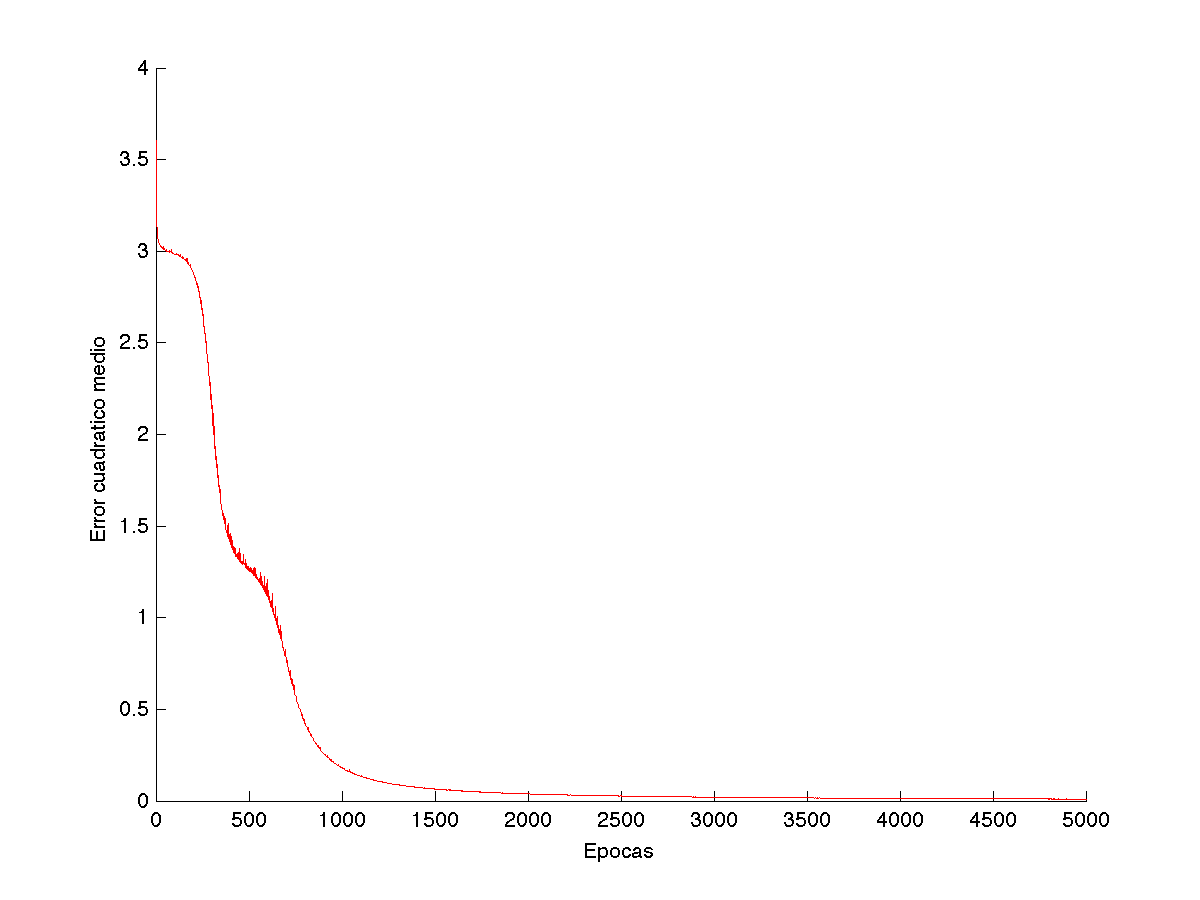
\includegraphics[scale=0.5]{images/sym_tanh_N5_eta002.png}
  \caption{Comparaci\'on del error para distintas funciones de activaci\'on con N = 5 en el problema de Simetri\'ia}
  \label{fig:symN5_TANH}
\end{figure}

\begin{figure}[!ht]
	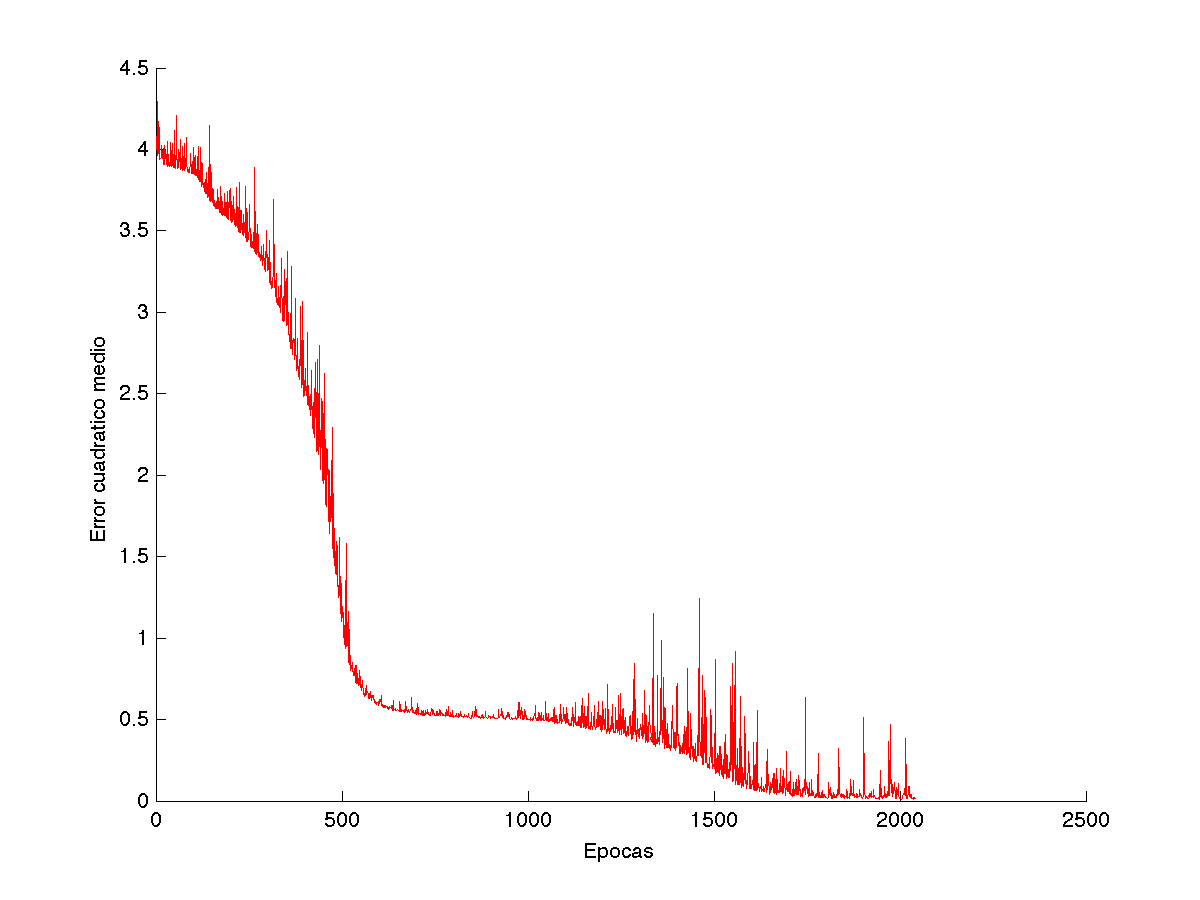
\includegraphics[scale=0.5]{images/par_tanh_N5_eta009.png}
  \caption{Comparaci\'on del error para distintas funciones de activaci\'on con N = 5 en el problema de Paridad}
  \label{fig:parN5_TANH}
\end{figure}

\begin{figure}[!ht]
	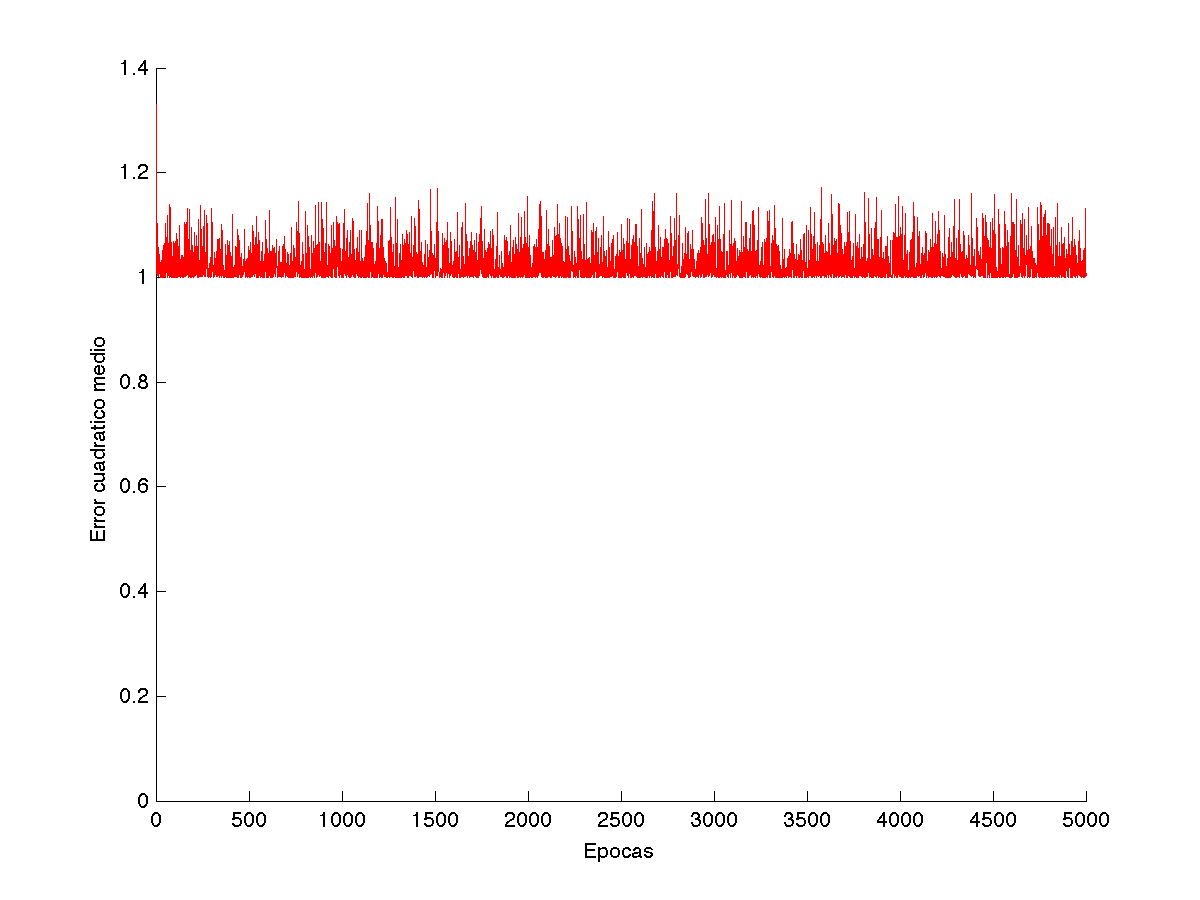
\includegraphics[scale=0.5]{images/sym_lineal_N3_eta02.png}
  \caption{Comparaci\'on del error para distintas funciones de activaci\'on en la \'ultima capa, con N = 3 en el problema de Simetr\'ia}
  \label{fig:symN3_LINEAL}
\end{figure}

\begin{figure}[!ht]
	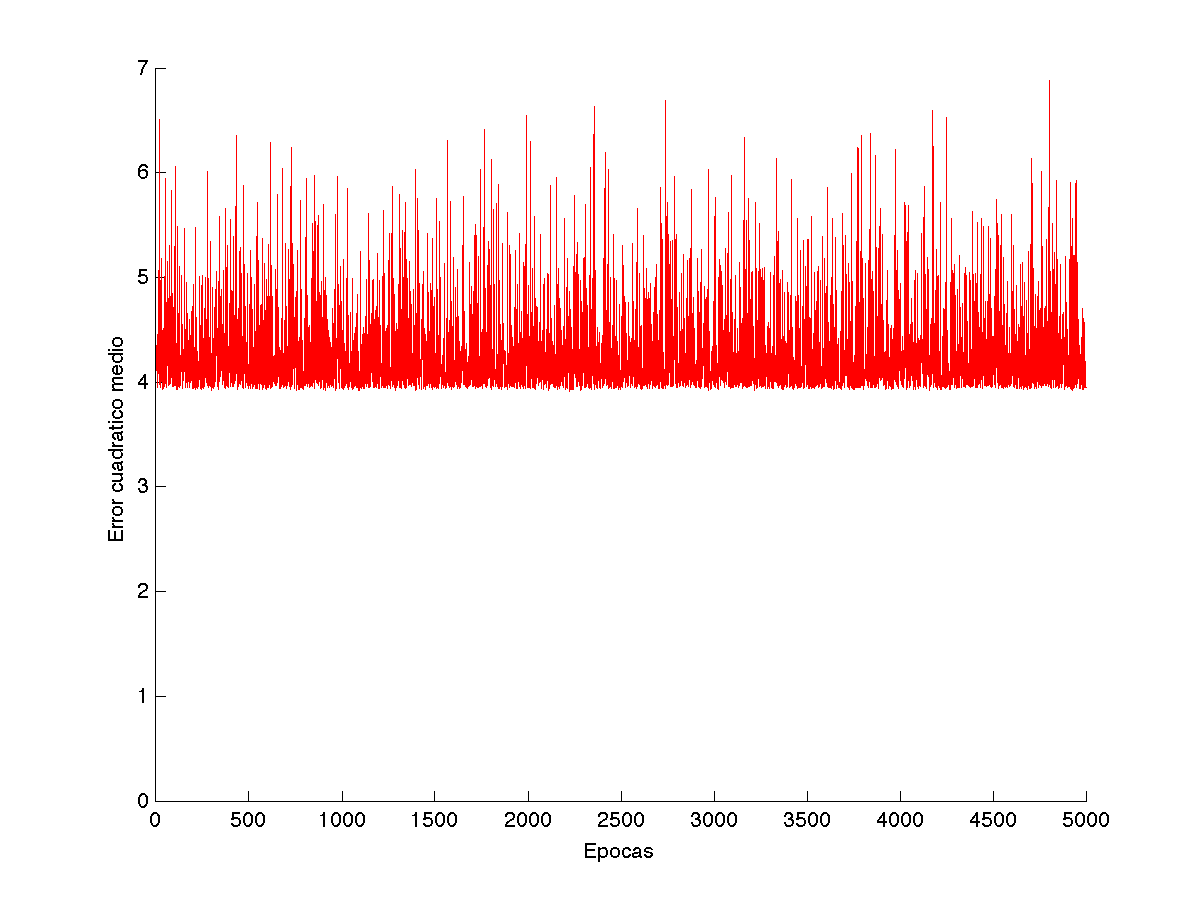
\includegraphics[scale=0.5]{images/par_lineal_N5_eta02.png}
  \caption{Comparaci\'on del error para distintas funciones de activaci\'on en la \'ultima capa, con N = 5 en el problema de Paridad}
  \label{fig:parN5_LINEAL}
\end{figure}

\begin{figure}[!ht]
	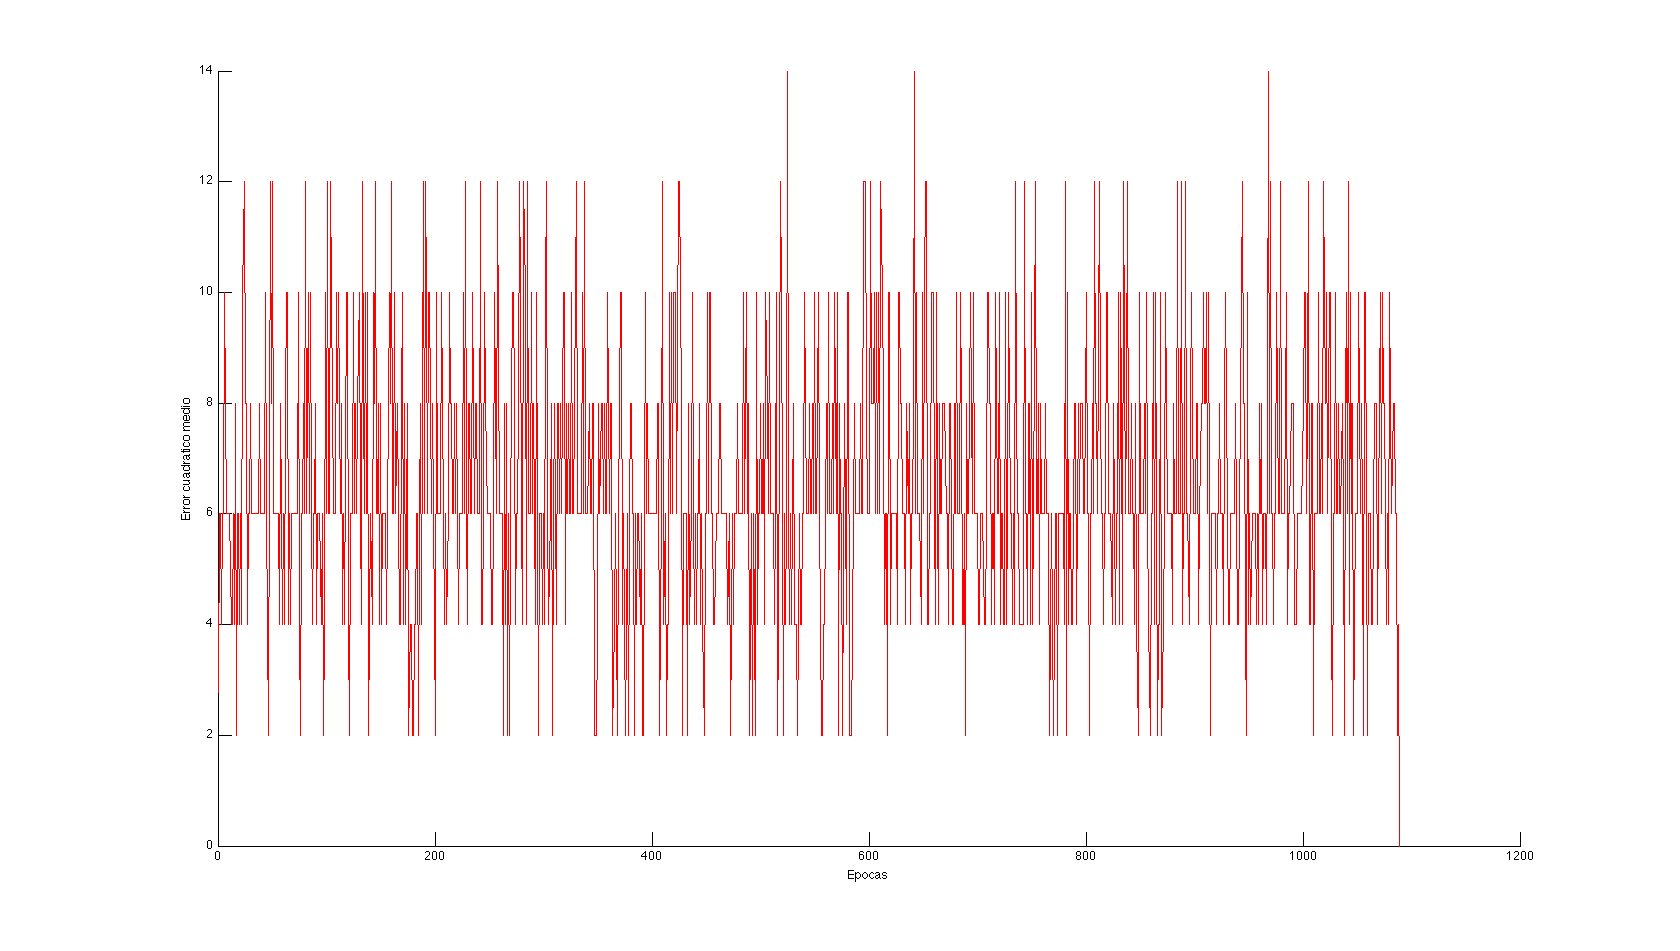
\includegraphics[scale=0.5]{images/par_step_N3_eta02.png}
  \caption{Comparaci\'on del error para distintas funciones de activaci\'on en la \'ultima capa, con N = 3 en el problema de Paridad}
  \label{fig:parN3_STEP}
\end{figure}

\begin{figure}[!ht]
	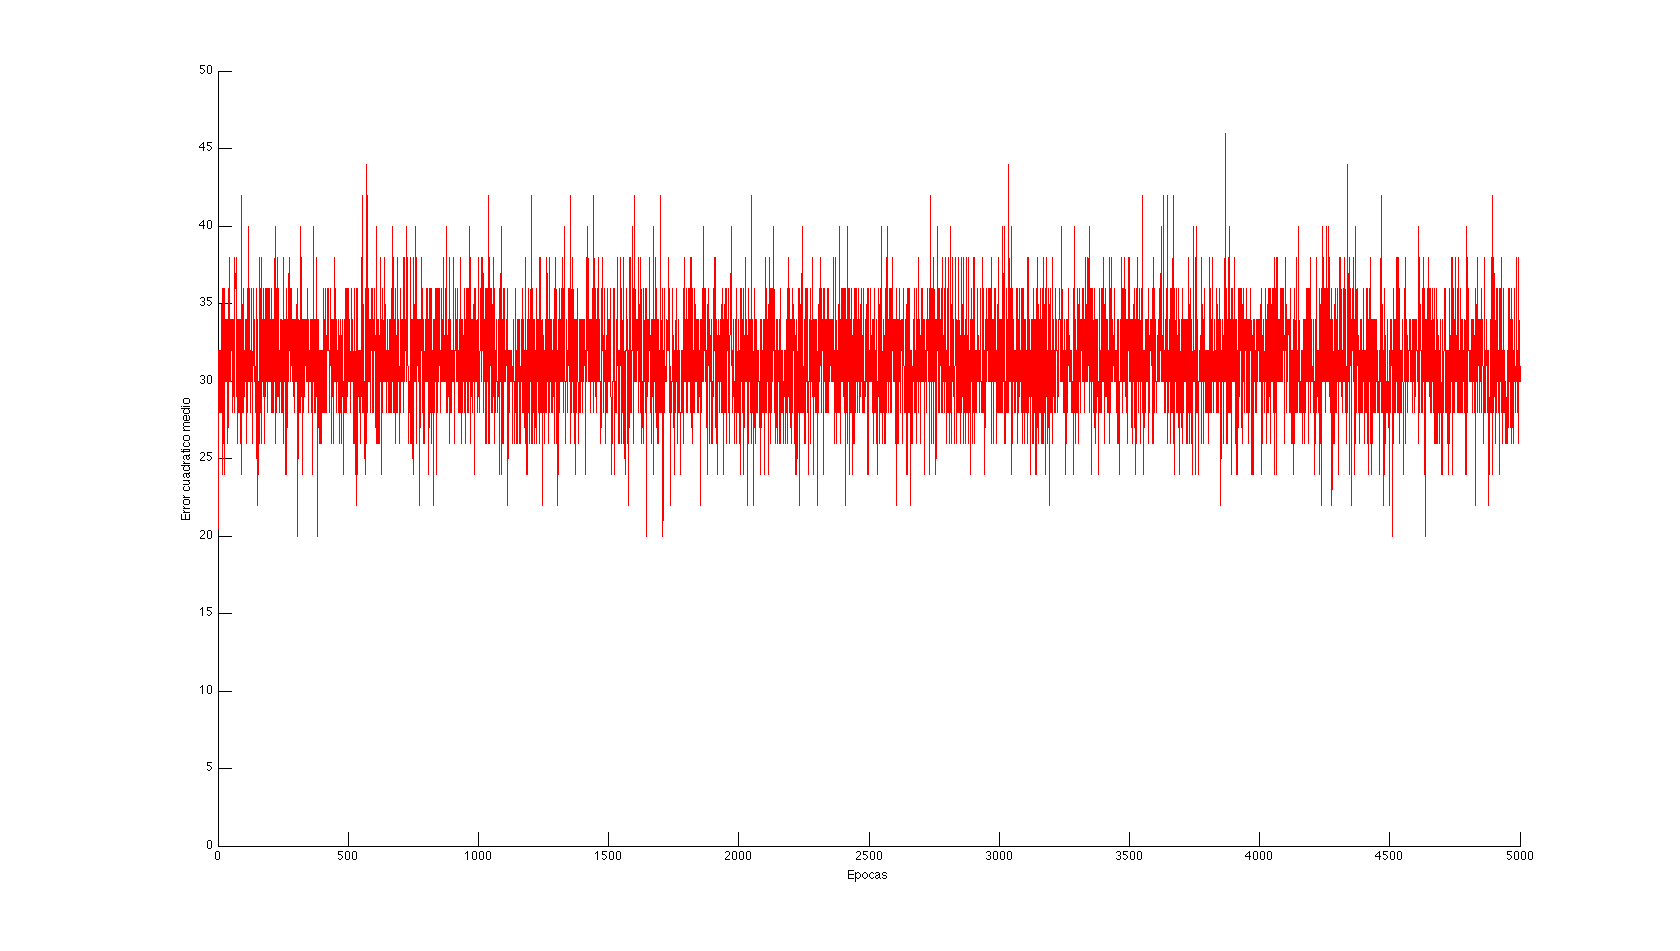
\includegraphics[scale=0.5]{images/par_step_N5_eta02.png}
  \caption{Comparaci\'on del error para distintas funciones de activaci\'on en la \'ultima capa, con N = 3 en el problema de Simetr\'ia}
  \label{fig:parN5_STEP}
\end{figure}


\end{document}